%%%%%%%%%%%%%%%%%%%%%%%%%%%%%%%%%%%%%%%%%
% Short Sectioned Assignment
% LaTeX Template
% Version 1.0 (5/5/12)
%
% This template has been downloaded from:
% http://www.LaTeXTemplates.com
%
% Original author:
% Frits Wenneker (http://www.howtotex.com)
%
% License:
% CC BY-NC-SA 3.0 (http://creativecommons.org/licenses/by-nc-sa/3.0/)
%
%%%%%%%%%%%%%%%%%%%%%%%%%%%%%%%%%%%%%%%%%

%----------------------------------------------------------------------------------------
%	PACKAGES AND OTHER DOCUMENT CONFIGURATIONS
%----------------------------------------------------------------------------------------

\documentclass[paper=a4, fontsize=11pt]{scrartcl} % A4 paper and 11pt font size

\usepackage[T1]{fontenc} % Use 8-bit encoding that has 256 glyphs
\usepackage{enumitem}
\usepackage{amsmath}
\usepackage{graphicx}
\usepackage{hyperref}
\usepackage{fourier} % Use the Adobe Utopia font for the document - comment this line to return to the LaTeX default
\usepackage[english]{babel} % English language/hyphenation
\usepackage{amsmath,amsfonts,amsthm} % Math packages

\usepackage{lipsum} % Used for inserting dummy 'Lorem ipsum' text into the template

\usepackage{sectsty} % Allows customizing section commands
\allsectionsfont{\centering \normalfont\scshape} % Make all sections centered, the default font and small caps

\usepackage{amsmath}

\usepackage{amssymb}

\usepackage{fancyhdr} % Custom headers and footers
\pagestyle{fancyplain} % Makes all pages in the document conform to the custom headers and footers
\fancyhead{} % No page header - if you want one, create it in the same way as the footers below
\fancyfoot[L]{} % Empty left footer
\fancyfoot[C]{} % Empty center footer
\fancyfoot[R]{\thepage} % Page numbering for right footer
\renewcommand{\headrulewidth}{0pt} % Remove header underlines
\renewcommand{\footrulewidth}{0pt} % Remove footer underlines
\setlength{\headheight}{13.6pt} % Customize the height of the header

%\numberwithin{equation}{section} % Number equations within sections (i.e. 1.1, 1.2, 2.1, 2.2 instead of 1, 2, 3, 4)
\numberwithin{figure}{section} % Number figures within sections (i.e. 1.1, 1.2, 2.1, 2.2 instead of 1, 2, 3, 4)
\numberwithin{table}{section} % Number tables within sections (i.e. 1.1, 1.2, 2.1, 2.2 instead of 1, 2, 3, 4)

\setlength\parindent{0pt} % Removes all indentation from paragraphs - comment this line for an assignment with lots of text

%----------------------------------------------------------------------------------------
%	TITLE SECTION
%----------------------------------------------------------------------------------------

\newcommand{\horrule}[1]{\rule{\linewidth}{#1}} % Create horizontal rule command with 1 argument of height

\title{	
\normalfont \normalsize 
\textsc{} \\ [25pt] % Your university, school and/or department name(s)
\horrule{0.5pt} \\[0.4cm] % Thin top horizontal rule
\huge Storage Systems\\ % The assignment title
\large Prof. Asadi \\
\Large Assignment \#1 - Due on Aban 2nd
\horrule{2pt} \\[0.5cm] % Thick bottom horizontal rule
}

\author{Nima Mohammadi} % Your name

\date{\normalsize nima.mohammadi@ut.ac.ir} 

\renewcommand{\floatpagefraction}{.99}%

\begin{document}

\maketitle % Print the title

\section{Simulating RAID with SimDisk}

We base our work on synthraid5.parv configuration file which corresponds to a RAID5 8+1. 
I noticed that "Storage capacity per device" for generators has been set to $16448064$, which seems to be wrong and outdated as the specifications for HP\_C3323A states that block count for this model has been corrected "from $2056008$ to $1743672$". Apparently the former value had been used for synthraid5.parv. 

I have tested two forks of DiskSim, one by Dirk Meister and the other by Western Digital. Meister\'s fork only run on Linux, but I managed to run WD\'s fork on OS X as well. I found out that WD\'s fork has oddly limited the maximum number of reqs to 200000, hardcoded in src/disksim\_simresult.h (\href{https://github.com/westerndigitalcorporation/DiskSim/blob/dc21ab0bd53af26ef1acd8b2b9f8dd842aaa338e/STABLE/DiskSim_Linux_Generic_2.01.016/src/disksim_simresult.h#L64}{+}).

\section{Synthetic Workload}
Three investigated \textit{request sizes}, namely small, medium and large, were sampled from a normal distribution $\mathcal{N}(4, 2)$, $\mathcal{N}(16, 2)$ and $\mathcal{N}(64, 2)$, respectively.

For each configuration, two synthetic workload generators are incorporated with identical settings. Probability of local accesses is set to $30\%$. Of all requests, $66\%$ of them are read accesses and $20\%$ are sequential.


\section{First Metric: Throughput}
As for the first unit of measurement we opted the throughput of the system, reported under "\textit{Overall I/O System Requests per second}" in DiskSim output log. How the throughput of these configurations is changed with respect to the req. size is depicted in Figure \ref{fig1}.

\begin{figure}
\begin{center}
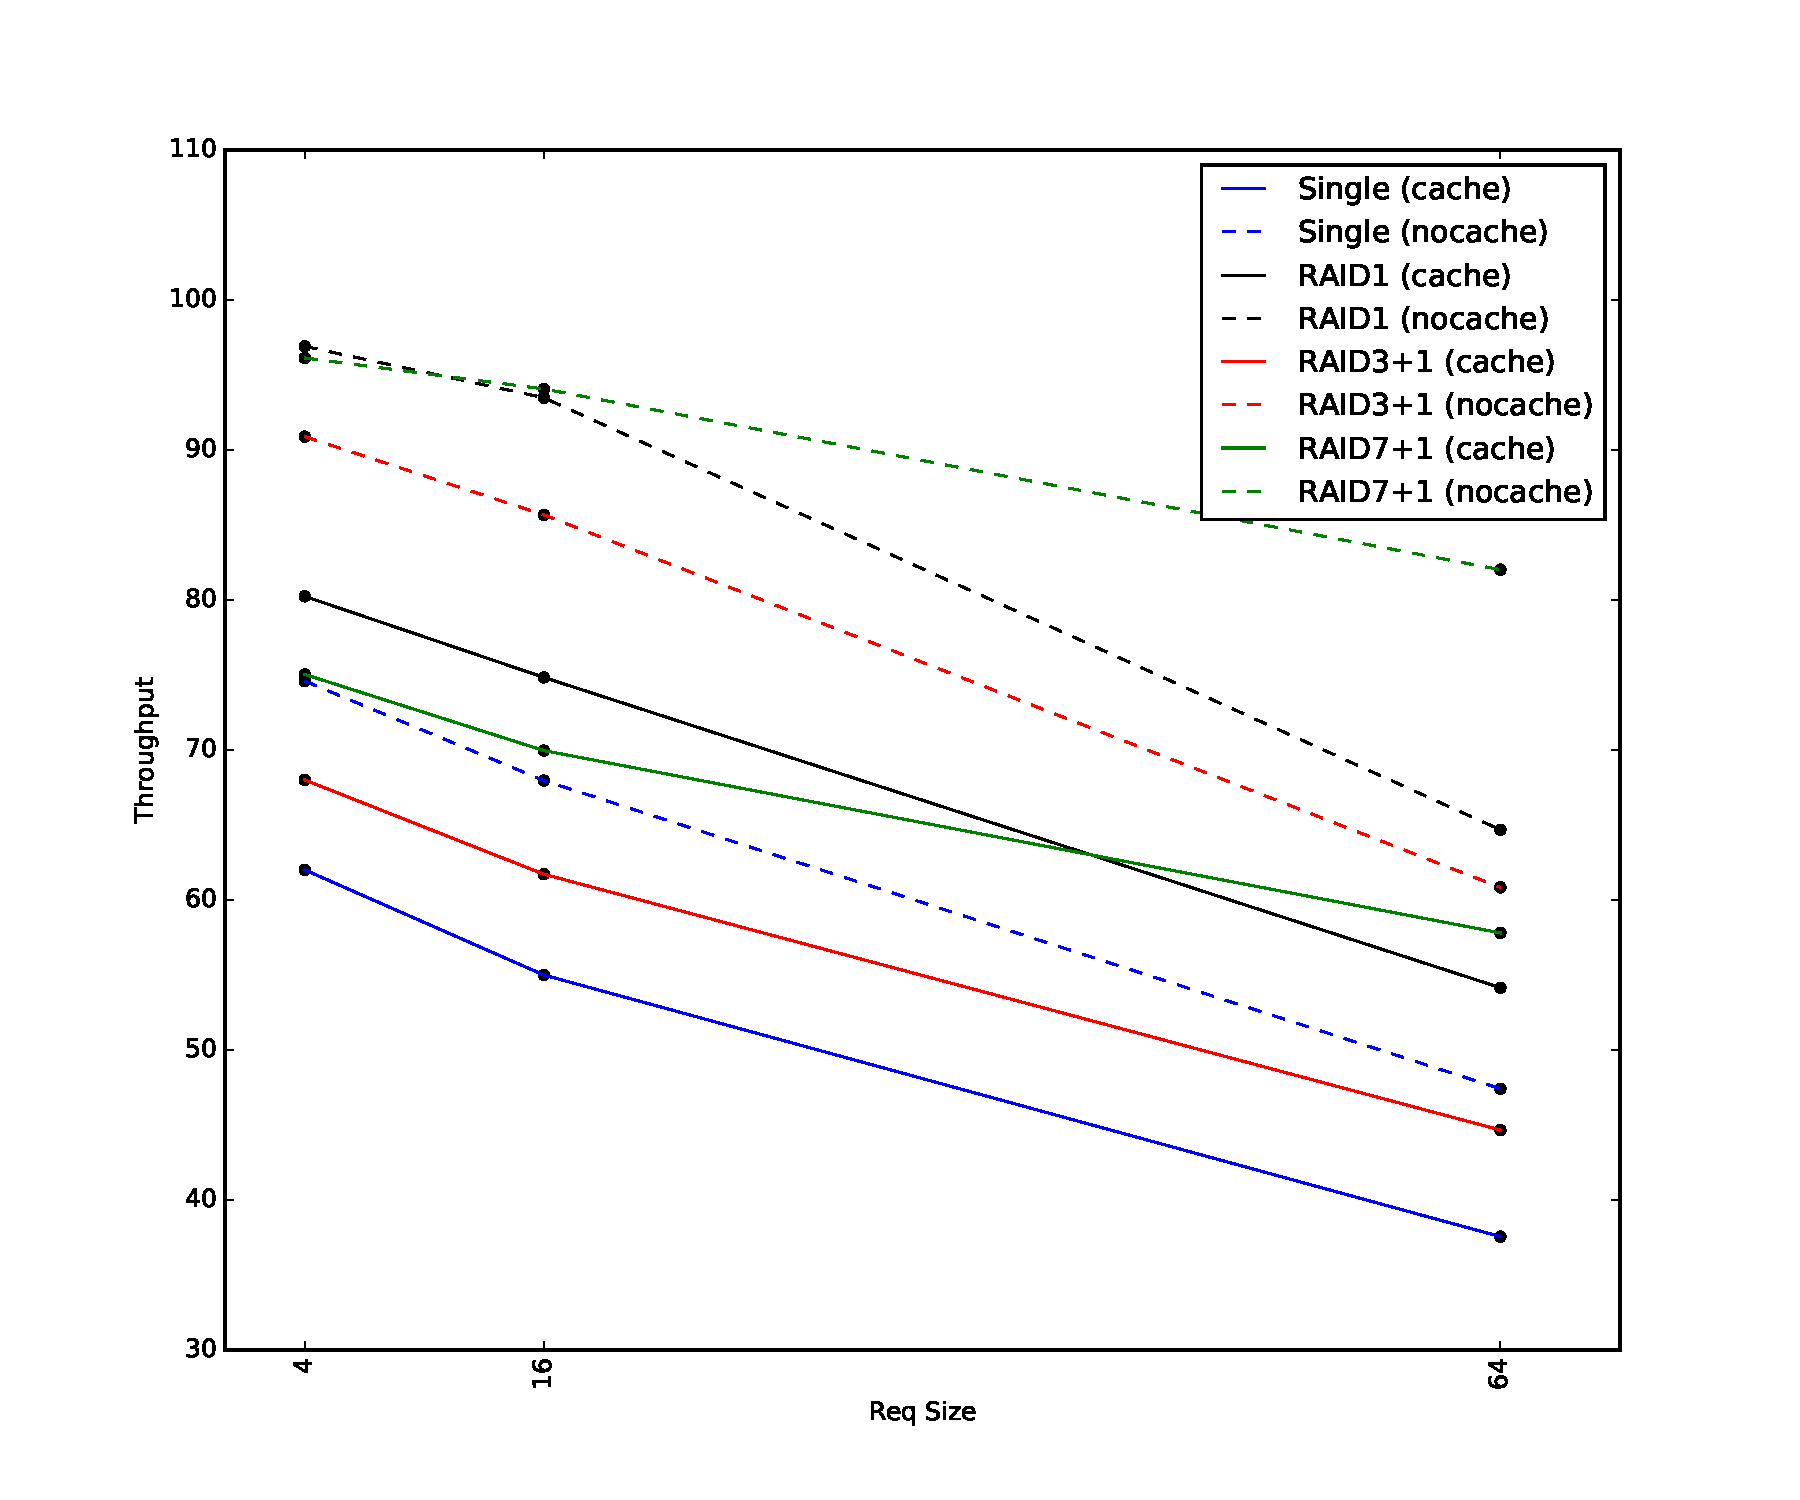
\includegraphics[width=14cm]{plot1.pdf}
\caption{Throughput of various configurations reported by DiskSim}
\label{fig1}
\end{center}
\end{figure}

\section{Second Metric: Average Response Time}
We chose average response time, reported under "\textit{Overall I/O System Response time average}" in DiskSim output log as the second criterion. How AvgRT of these configurations is changed with respect to the req. size is depicted in Figure \ref{fig2}.

\begin{figure}
\begin{center}
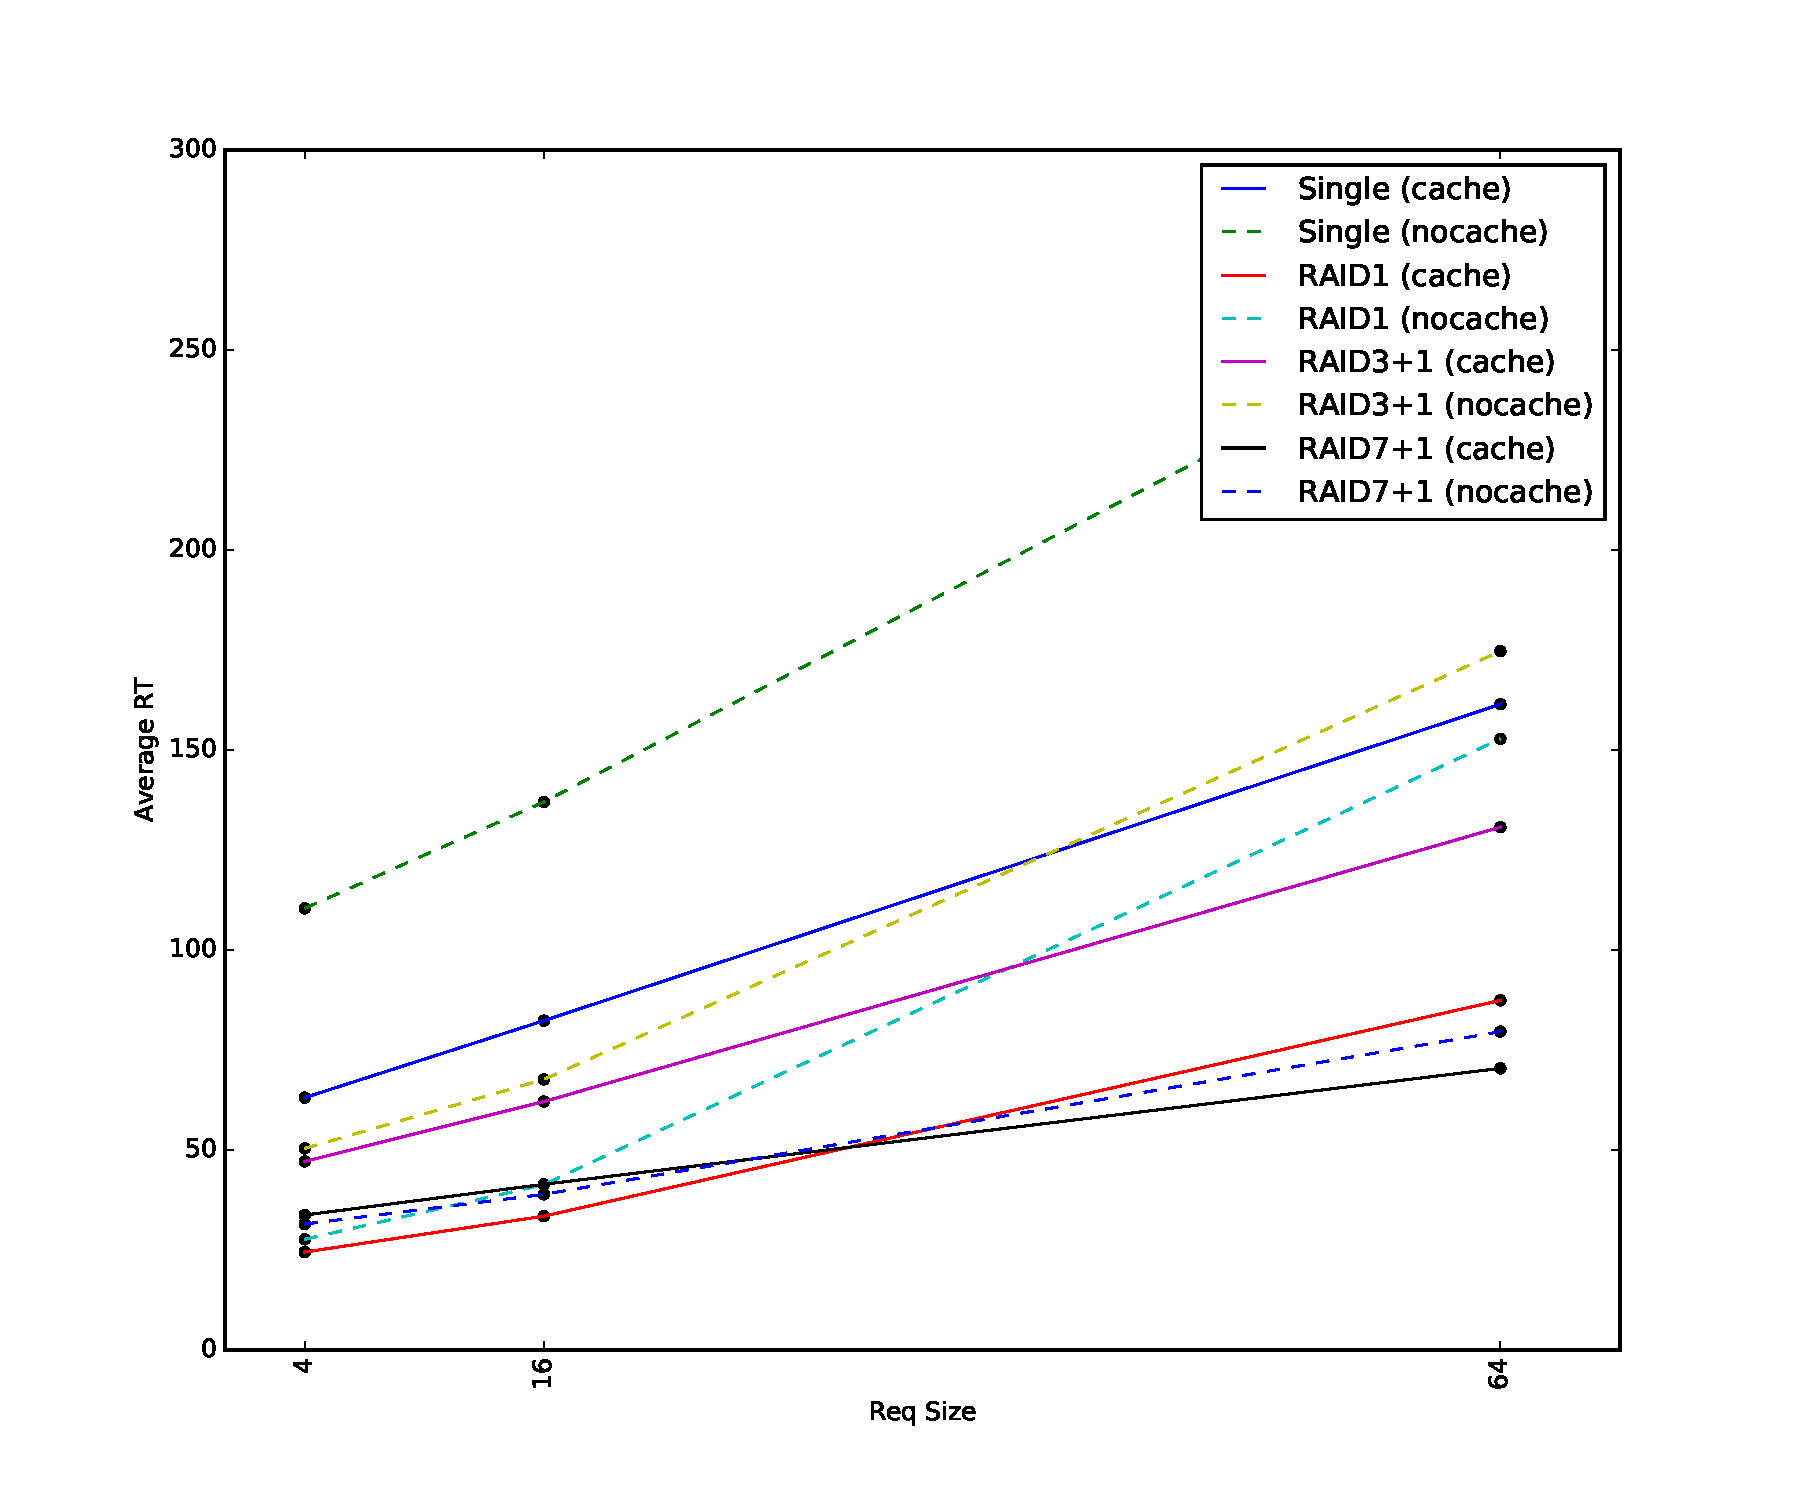
\includegraphics[width=14cm]{plot2.pdf}
\caption{Average Response Time of various configurations reported by DiskSim}
\label{fig2}
\end{center}
\end{figure}

\section{Observations}
As shown by Figure \ref{fig2}, fastest Avg. RT for small requests belongs to RAID1, which comes to no surprise as this configuration omits any redundancy and makes use of a very simple controller which divides the loads on two disks. However, as expected, a RAID configuration with more data disks (i.e. RAID 7+1) outperformed RAID1 for requests of larger sizes. That is not the case for small req. sizes, probably due to the overhead of incorporating seven disks to acquire a rather small chunk of data. As for the worst case, the single disk scenario, and more specifically the configuration without caching, is without a doubt slower. Moreover, I can not come up with an explanation as to why RAID3+1 does not lie between the two other RAID configurations. 

Disclaimer: My experiments showed inferior throughput for cases with a caching mechanism (i.e. disksim\_cachemem) compared with no cache. I told this to Ms. Ahmadian and discussed it with Mr. Tarihi, who dissed DiskSim for its cache implementation. I have tested many possible scenarios, from increasing cache size, changing read and write schemes of cache, enabling prefetching, changing replacement policy to changing the locality of the synthetic workload, but to no avail.

Regardless of throughputs of various configurations (Fig. \ref{fig1}) compared to each other, we can see that throughput of RAID7+1 has a less steep decline as the request size grows, compared to other schemes. 

\section{Tables}

\begin{table}[h]
\centering
\caption{Throughputs}
\label{reptab1}
\begin{tabular}{|l|l|l|l|}
\hline
              & \textbf{Small Req.} & \textbf{Medium Req.} & \textbf{Large Req.} \\ \hline
Single (cache) & 62.007962                   & 54.998343                    & 37.556862                   \\ \hline
Single (nocache) & 74.595594                   & 67.961751                    & 47.418344                   \\ \hline
RAID1 (cache) & 80.245812                   & 74.839183                    & 54.152121                   \\ \hline
RAID1 (nocache) & 96.909472                   & 93.480399                    & 64.680562                   \\ \hline
RAID3+1 (cache) & 68.005914                   & 61.719199                    & 44.663290                   \\ \hline
RAID3+1 (nocache) & 90.890062                   & 85.674496                    & 60.838577                   \\ \hline
RAID7+1 (cache) & 75.039194                   & 69.962464                    & 57.806363                   \\ \hline
RAID7+1 (nocache) & 96.135604                   & 94.068864                    & 82.021575                   \\ \hline

\end{tabular}
\end{table}

\begin{table}[h]
\centering
\caption{Average Response Times}
\label{reptab2}
\begin{tabular}{|l|l|l|l|}
\hline
              & \textbf{Small Req.} & \textbf{Medium Req.} & \textbf{Large Req.} \\ \hline
Single (cache) & 63.087211                   & 82.329793                    & 161.435756                   \\ \hline
Single (nocache) & 110.414437                   & 137.002508                    & 261.629921                   \\ \hline
RAID1 (cache) & 24.477941                   & 33.459932                    & 87.410663                   \\ \hline
RAID1 (nocache) & 27.666542                   & 41.368288                    & 152.808413                   \\ \hline
RAID3+1 (cache) & 47.150294                   & 62.105883                    & 130.703169                   \\ \hline
RAID3+1 (nocache) & 50.400269                   & 67.642395                    & 174.720636                   \\ \hline
RAID7+1 (cache) & 33.742821                   & 41.424422                    & 70.416513                   \\ \hline
RAID7+1 (nocache) & 31.485917                   & 38.923116                    & 79.612017                   \\ \hline


\end{tabular}
\end{table}

\end{document}
